\documentclass[12pt]{article}
%\documentclass[12pt, letterpaper, twoside]{article}
\usepackage{graphicx}
\usepackage{xcolor}
\usepackage{subcaption}
\usepackage{hyperref}
\definecolor{linkcolour}{rgb}{0,0,1}
\hypersetup{colorlinks=true, urlcolor=linkcolour, linkcolor=linkcolour, linkbordercolor=linkcolour, pdfborderstyle={/S/U/W 1}} 
\urlstyle{same}

\usepackage{setspace} 
\singlespacing

\usepackage{geometry}
\geometry{margin=1in}

\setlength\parindent{0pt}

\begin{document}
\title{Bike-Share Case Study}
\date{}
\maketitle

This report provides the results and step-step explanation of the data analysis performed for a bike sharing case-study. The data belongs to a bike-sharing company that has two kinds of users: annual members and casual riders. The goal of the case-study was to identify how annual members and casual riders use the bikes differently in order to help the stake-holders decide whether or not to target converting casual riders into annual members in the next marketing campaign. The data about the bike-rides used in this case-study was between January-November 2023, each month was stored in a csv file, and was downloaded from \url{https://divvy-tripdata.s3.amazonaws.com/index.html}. 

\section*{Data cleaning:}
The code that was used to perform the data cleaning can be found in the Jupyter Notebook \href{https://github.com/SummerKassem/BikeShareCS/blob/main/Code/cleaning.ipynb}{cleaning.ipynb}. Here are the main functions and what they do.
\begin{itemize}
	\item \textit{read\_data}:\\
	Here the csv files are read and stored into a dictionary called “data”. Each element in the dictionary has a key (the name of the month) and a value (the panada dataframe that holds the csv entries). This way the data for each corresponding month can be easily accessed by using the month as the key (e.g. data[“February”] retrieves the dataframe that holds the entries from February). Below we can see the first 5 entries of bike rides from February:
	\begin{figure}[h]
	\hspace{-1.8cm}
	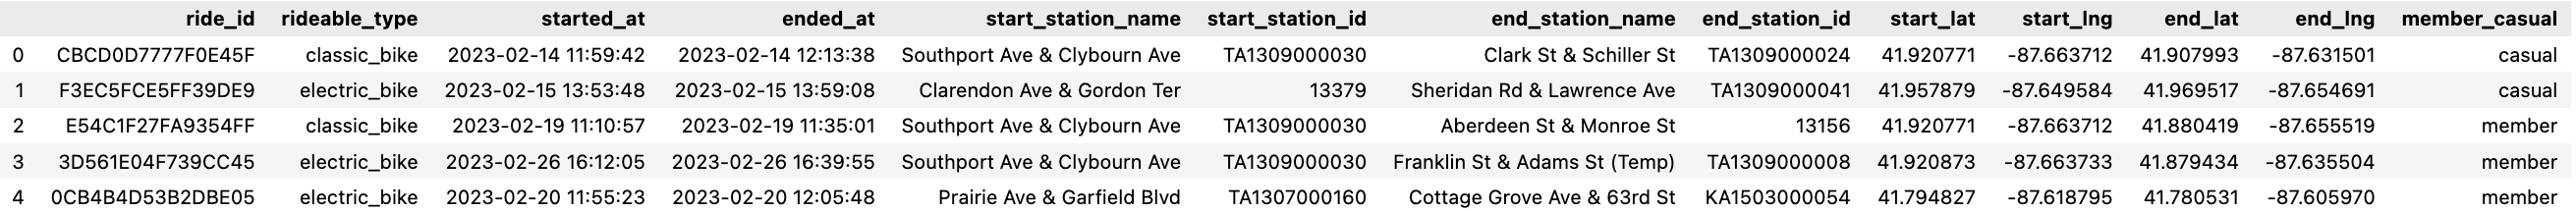
\includegraphics[width=8 in, height = 2 in]{img1.png}
	\end{figure}
	
	\item \textit{check\_entries}:\\
	This method performs a few preliminary calculations. It finds the number of entries per file as well as the number of columns. From these it calculates the total number of bike rides in the data set. There is also an option within the method to remove duplicates. Therefore, the method is first called with the remove duplicates option deactivated, in order to get a preliminary feel of the dataset, how big it is, how the entires varies across the months. And then the method is called again with the remove duplicates option activated. The results are then written to output files which are shown below. 
	
	\begin{figure}[h]
	\centering
	\begin{subfigure}{.4\textwidth}
	\hspace{0.5 in}
		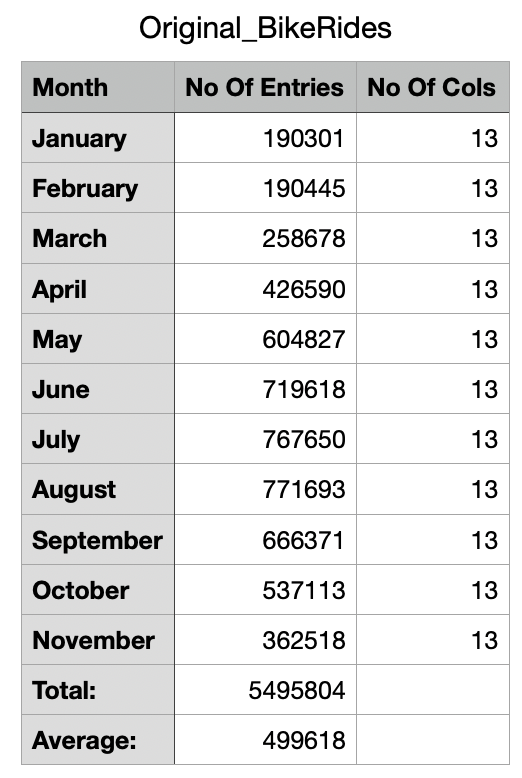
\includegraphics[scale=0.5]{img2.png}
	\end{subfigure}
	\begin{subfigure}{.4\textwidth}
	\hspace{0.5 in}
		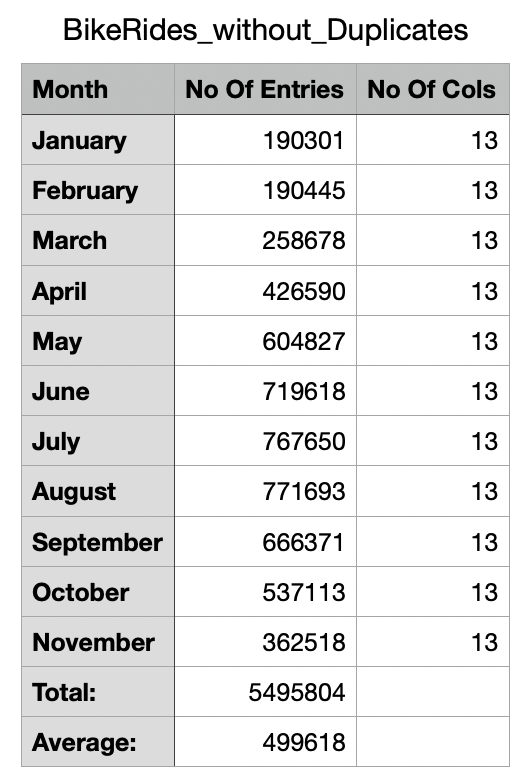
\includegraphics[scale=0.5]{img3.png}
	\end{subfigure}
	\end{figure}
	
On the left is the result of running the method without removing duplicates, and on the right is the result after removing duplicates. We can see that all the files have the same number of columns. So that is a good preliminary check on the consistency of the data across the months. In total the dataset contains 5.5 Million entries, with an average of 500,000 entries per month. So the dataset is relatively large. The number of entries before and after removing duplicates are identical, therefore the original dataset did not have any duplicates.
	
\end{itemize} 

\end{document}